% !TeX encoding=utf8
% !TeX spellcheck = en-US

\chapter{Evaluation}

The result of the algorithm is a set of user ids that are predicted destination nodes, given a specific source node. These are recommended users that the specified user might be interested in following. 

\section{Evaluation Metrics}

Each method described above in section (PROPER SECTION CITATION) is evaluated using the same evaluation metrics for comparison.

\subsection{Precision}

\subsection{HitRatio@k (Recall)}

\subsection{F-Measure}


\begin{table}[t]
\caption{Evaluation metrics for cross fold validation runs with varying parameters. K is number of neighbors allowed to vote. N is number of predicted links. Precision and accuracy are evaluation metrics, expressed in percentages. Random is the probability of at least one of the N links being relevant if N links are chosen at random.}
\label{results}
\vskip 0.15in
\begin{center}
\begin{small}
\begin{sc}
\begin{tabular}{rrccr}
\hline
k & n & Precision (\%) & Accuracy (\%) & Random (\%) \\
\hline
5      & 25 & 0.61 & 15.0 & 0.0046\\
5      & 50 & 0.18 & 8.0 & 0.0093 \\
5      & 100&0.19 & 15.0 & 0.0185\\
10    & 25 & 0.16& 4.0 & 0.0046\\
10    & 50 & 0.14 & 7.0 & 0.0093\\
10    & 100&0.19 & 18.0 & 0.0185 \\
25    & 25 & 0.24 & 6.0  & 0.0046\\
25    & 50 & 0.12 & 6.0  & 0.0093\\
25    &100&0.11 & 11.0  & 0.0185\\  
50    & 25 &0.12 & 3.0 & 0.0046\\
50    & 50 & 0.14 & 7.0  & 0.0093\\
50    &100& 0.10 & 0.10  & 0.0185\\
100 & 25 & 0.28 & 7.0  & 0.0046\\
100 & 50 & 0.16 & 8.0  & 0.0093\\
100 &100& 0.05 & 5.0  & 0.0185\\
1000&25&0.32 & 8.0  & 0.0046\\
1000&50&0.24& 12.0  & 0.0093\\
1000&100&0.14&14.0  & 0.0185\\
2000&25&0.24&6.0 & 0.0046\\
2000&50&0.18&9.0 & 0.0093\\
2000&100&0.10&10.0  & 0.0185\\
\hline
\end{tabular}
\end{sc}
\end{small}
\end{center}
\vskip -0.1in
\end{table}

\begin{table}[hb]
\centering
\small\renewcommand{\arraystretch}{1.4}  
\captionabove{Numbers of Computers in the department, By Type.}
\label{tab:Computers}
\begin{tabular}{lr}
\hline
Mac (Apple)    & 2  \\
Windows XP, 7  & 60 \\
Linux (Server) & 10 \\
\hline
\end{tabular}
\end{table}

\Cref{tab:IsingModel} on \cpageref{tab:IsingModel} demonstrate the creation of a pleasant appearing table, which helps to read the table without attracting to much attention by the use of shaded colors. The caption uses the additional short caption in square brackets \texttt{[ ]}, which is used in the list of tables, see \cpageref{sec:lot}.

\begin{table}[ht]
\centering
\small\renewcommand{\arraystretch}{1.4}  
\rowcolors{1}{tablerowcolor}{tablebodycolor}
%
\captionabove[Evaluation results - Jaccard]{Evaluation results for Jaccard similarity, for various values of $N$, where $N$ is the number of predictions generated for each user.}
\label{results_jaccard}
%
\begin{tabularx}{0.5\textwidth}{lXXX}
\hline
\rowcolor{tableheadcolor}
$N$ & HitRatio@$N$ & Precision & F-Measure \\
\hline
5 & 0.0494 & 0.0115 & 1.2 \\
10 & 0.0329 & 0.0039 & 1.2 \\
20 &0.0409 & 0.0025 & 1.2 \\
40 & 0.0389 & 0.0011 & 1.2 \\
50 & 0.0392 & 0.0010 & 1.2 \\
75 & 0.0285 & 5.0994 & 1.2 \\
\hline
\end{tabularx}
\end{table}

\begin{table}[ht]
\centering
\small\renewcommand{\arraystretch}{1.4}  
\rowcolors{1}{tablerowcolor}{tablebodycolor}
%
\captionabove[Evaluation results - Triadic Closeness]{Evaluation results for Triadic Closeness, for various values of $N$, where $N$ is the number of predictions generated for each user.}
\label{results_jaccard}
%
\begin{tabularx}{0.5\textwidth}{lXXX}
\hline
\rowcolor{tableheadcolor}
$N$ & HitRatio@$N$ & Precision & F-Measure \\
\hline
5 & 0.0364 & 0.0115 & 1.2 \\
10 & 0.0410 & 0.0039 & 1.2 \\
20 & 0.0479 & 0.0025 & 1.2 \\
40 & 0.0526 & 0.0011 & 1.2 \\
50 & 0.0392 & 0.0010 & 1.2 \\
75 & 0.0522 & 5.0994 & 1.2 \\
100 & 0.0392 & 0.132 & 1.2 \\
250 & 0.0285 & 0.3242 & 1.2 \\
500 & 0.0135 & 0.3234 & 1.2 \\
1000 & 0.033 & 0.3211 & 1.2 \\
5000 & 0.0166 & 0.4431 & 1.2 \\
\hline
\end{tabularx}
\end{table}

\begin{table}[ht]
\centering
\small\renewcommand{\arraystretch}{1.4}  
\rowcolors{1}{tablerowcolor}{tablebodycolor}
%
\captionabove[Evaluation results - Adaptive Ensemble]{Evaluation results for Adaptive Ensemble, for various values of $N$, where $N$ is the number of predictions generated for each user.}
\label{results_jaccard}
%
\begin{tabularx}{0.5\textwidth}{lXXX}
\hline
\rowcolor{tableheadcolor}
$N$ & HitRatio@$N$ & Precision & F-Measure \\
\hline
5 & 0.0364 & 0.0115 & 1.2 \\
10 & 0.0410 & 0.0039 & 1.2 \\
20 & 0.0479 & 0.0025 & 1.2 \\
40 & 0.0526 & 0.0011 & 1.2 \\
50 & 0.0392 & 0.0010 & 1.2 \\
75 & 0.0522 & 5.0994 & 1.2 \\
100 & 0.0392 & 0.132 & 1.2 \\
250 & 0.0285 & 0.3242 & 1.2 \\
500 & 0.0135 & 0.3234 & 1.2 \\
1000 & 0.033 & 0.3211 & 1.2 \\
5000 & 0.0166 & 0.4431 & 1.2 \\
\hline
\end{tabularx}
\end{table}




\begin{figure}[htb]
  \centering
  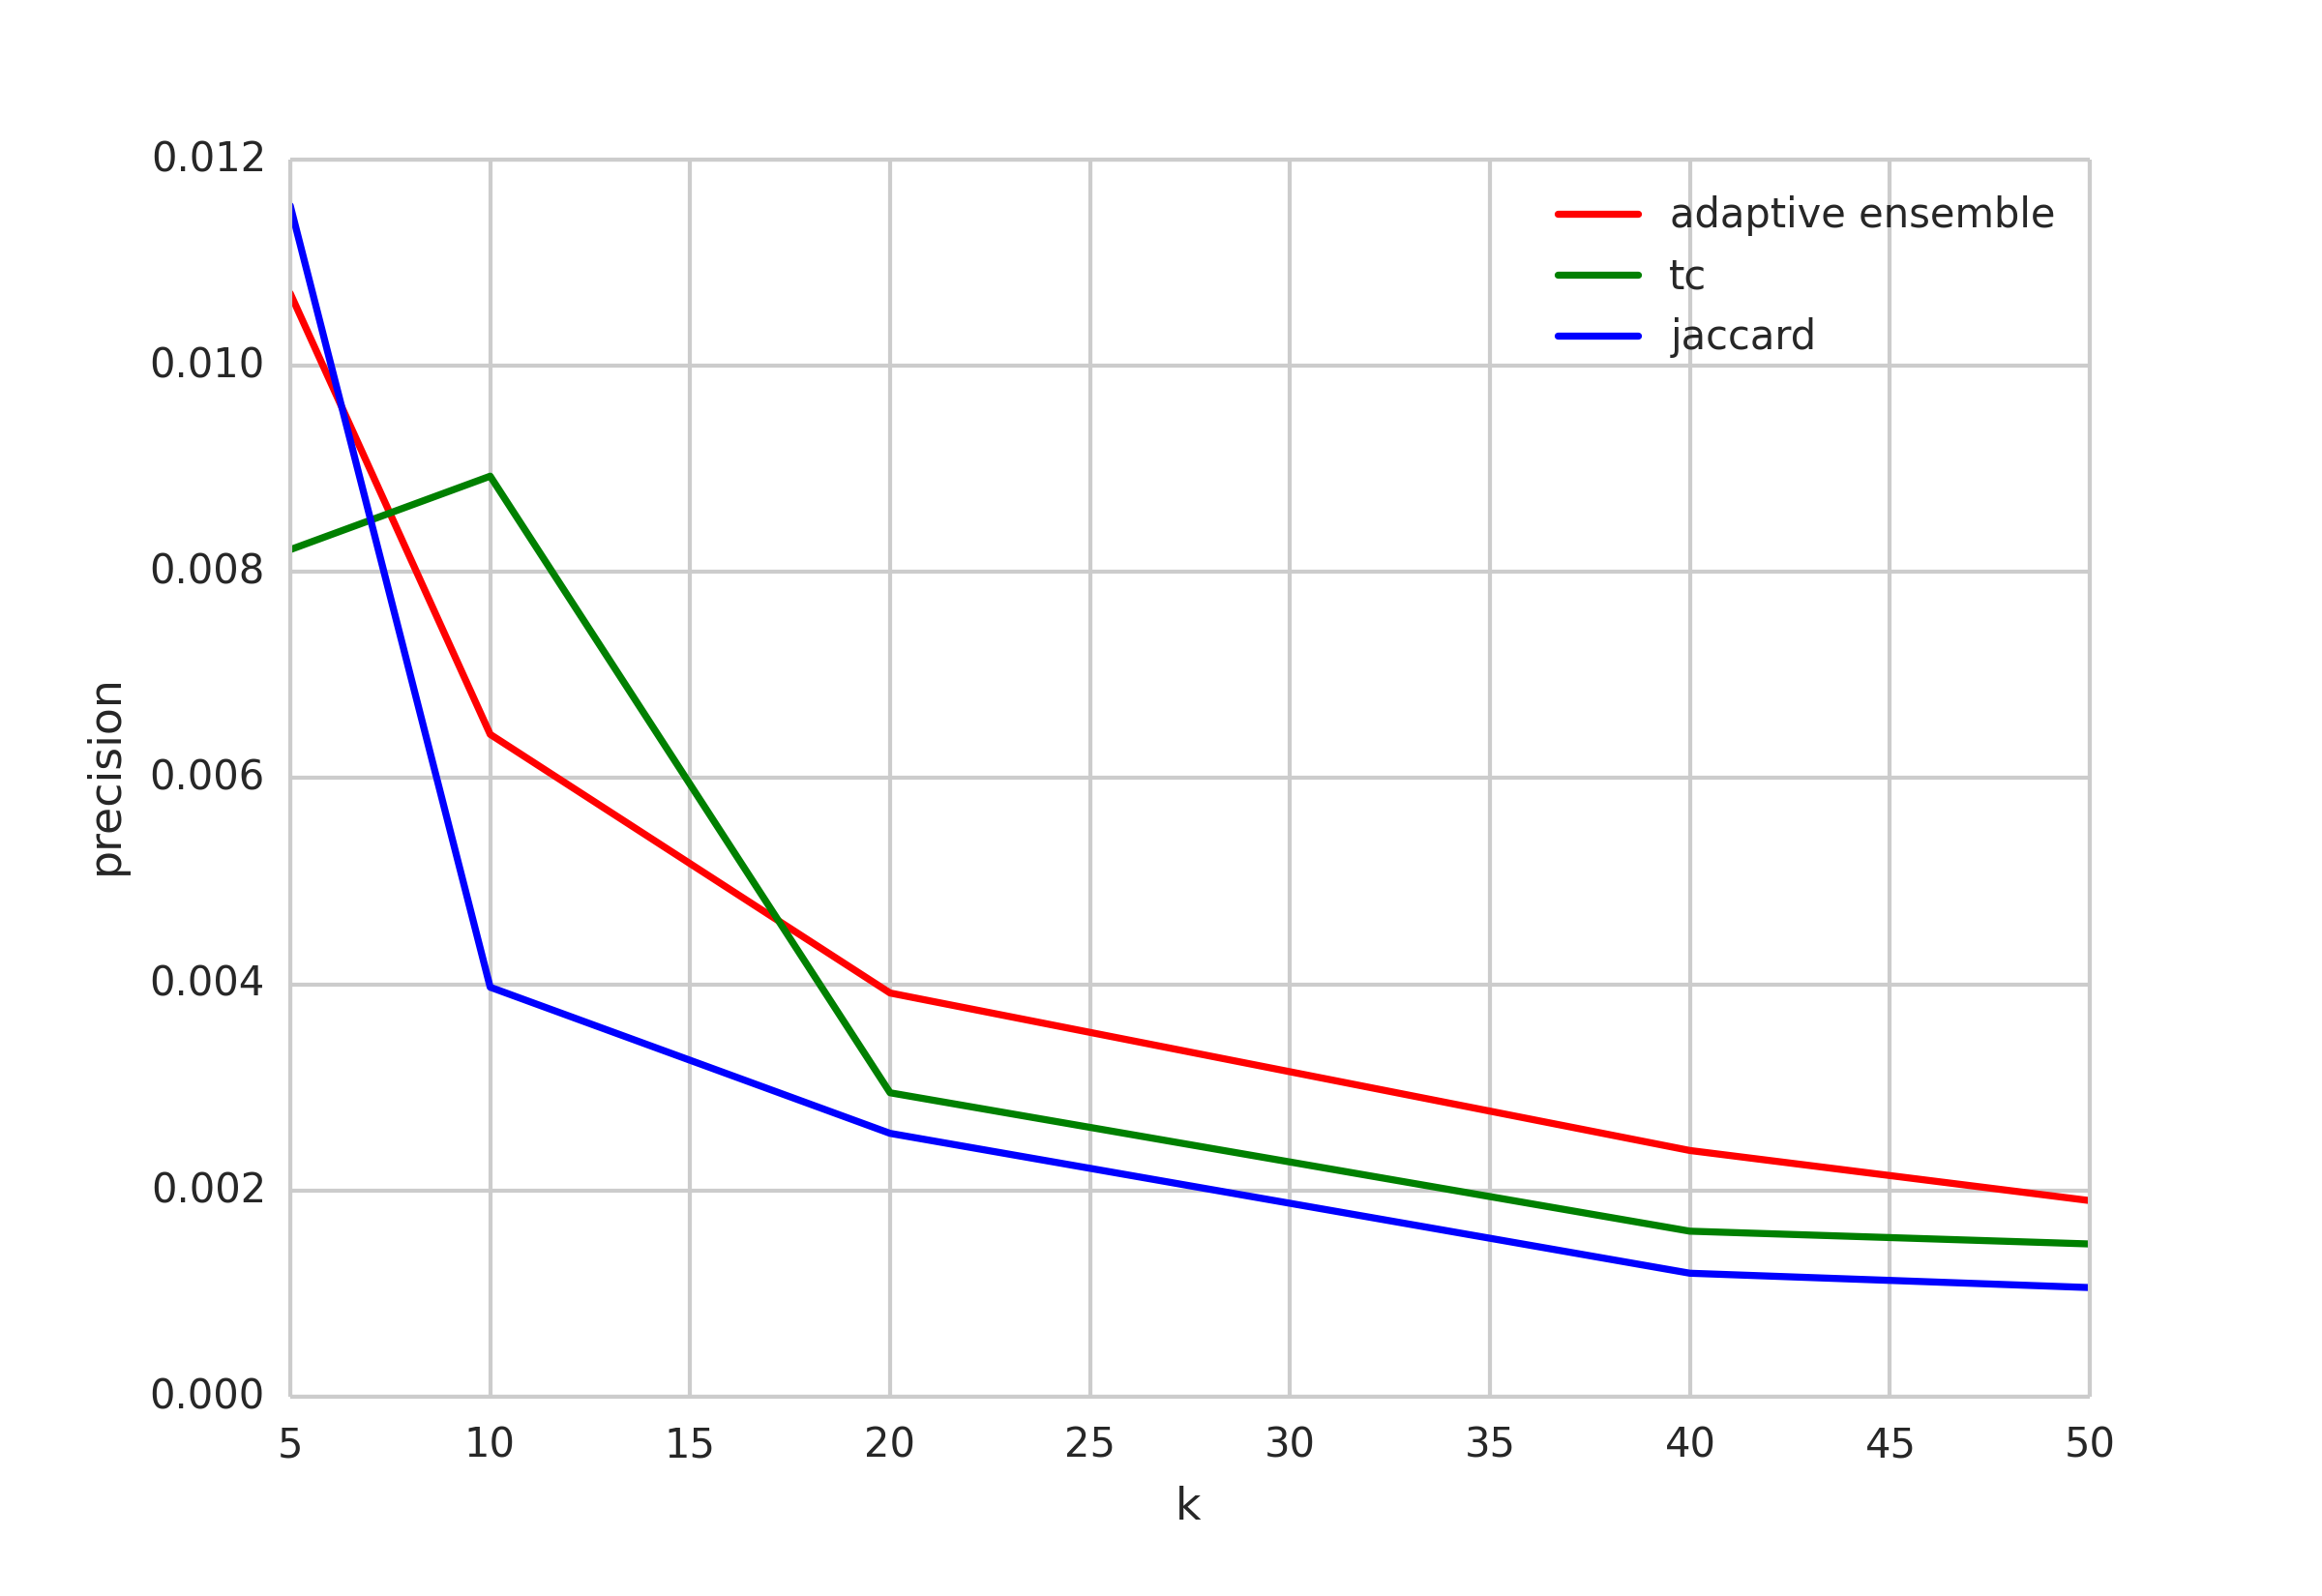
\includegraphics[width=0.75\textwidth]{images/precision_line.png}
  \caption[Test image for television]{Test image for television (Origin of the image: \url{http://de.wikipedia.org/wiki/Testbild}).}
  \label{fig:example:figure}
\end{figure}

All possibilities of grouping pictures side by side, on top or in matrices can be realized. Each subfigure is created in the same way as a graphic inside a figure, just enclosed by a figure environment, as shown in \cref{fig:example:subfigures}.
\begin{figure}[htb]
  \begin{subfigure}[b]{.45\linewidth}
    \centering
    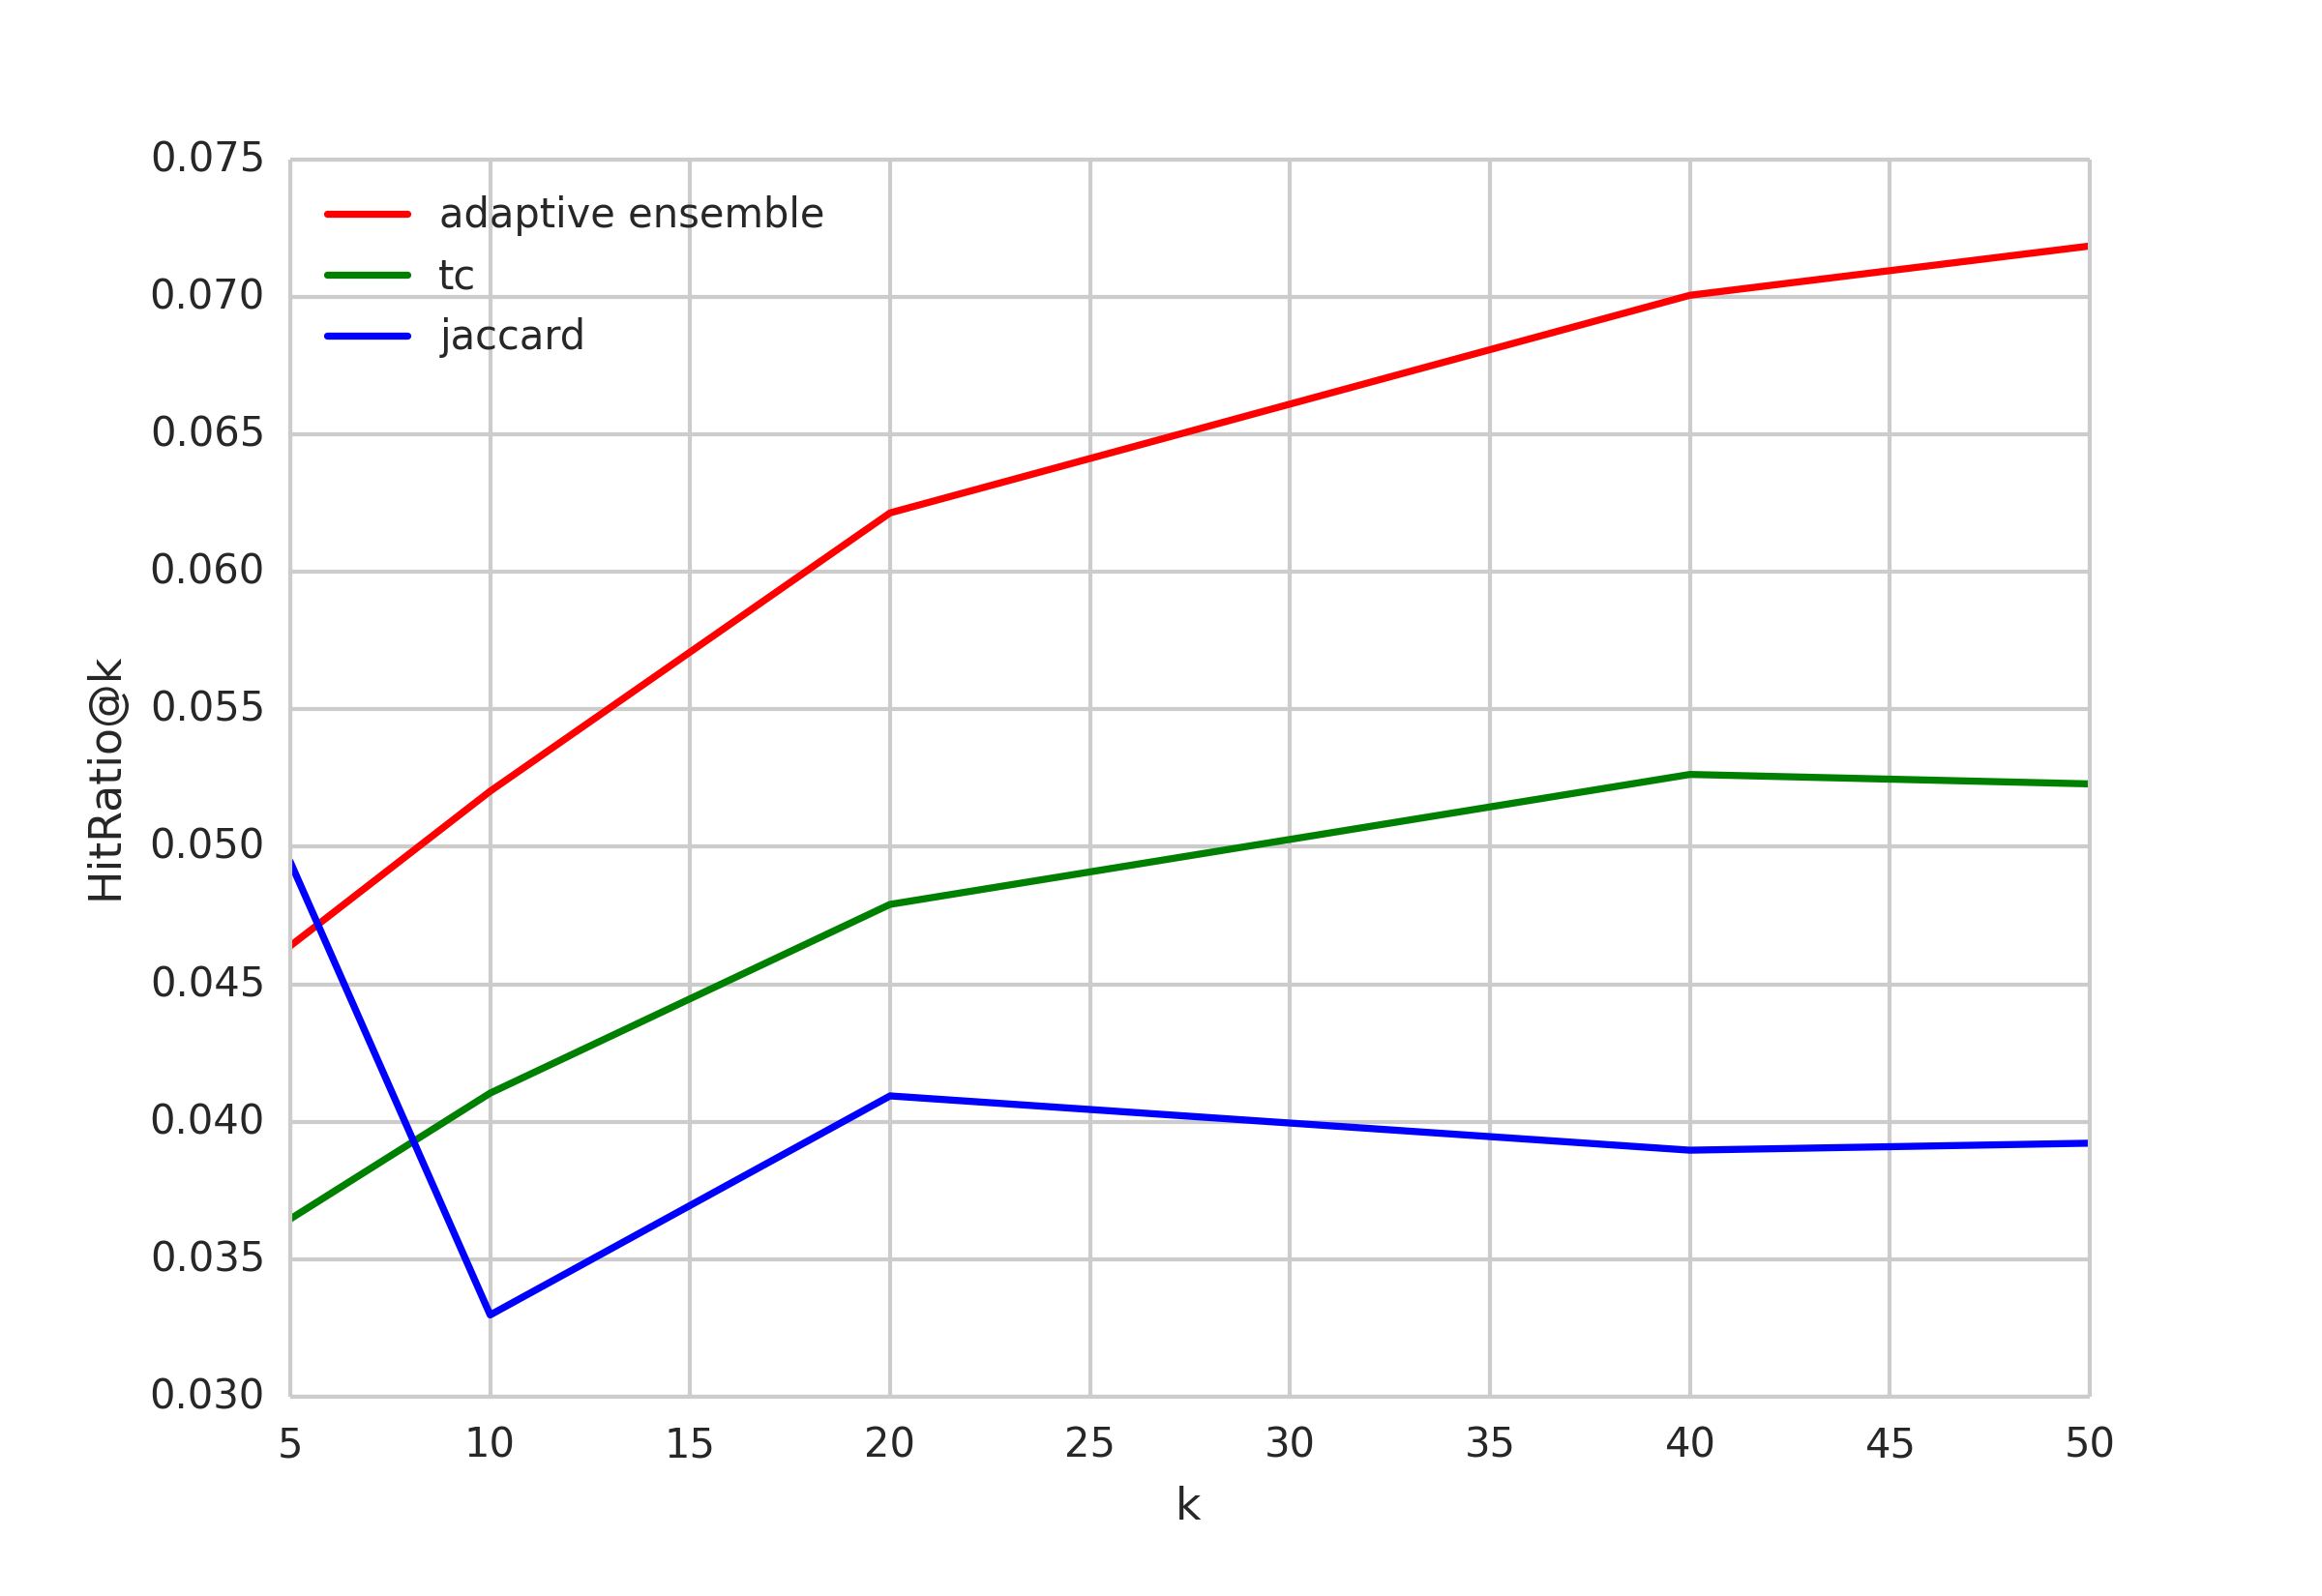
\includegraphics[width=0.95\linewidth]{images/hitratio_line.png}
    \caption{The first subfigure.}
    \label{fig:example:subfigures:a}
  \end{subfigure}%
  \begin{subfigure}[b]{.45\linewidth}
    \centering
    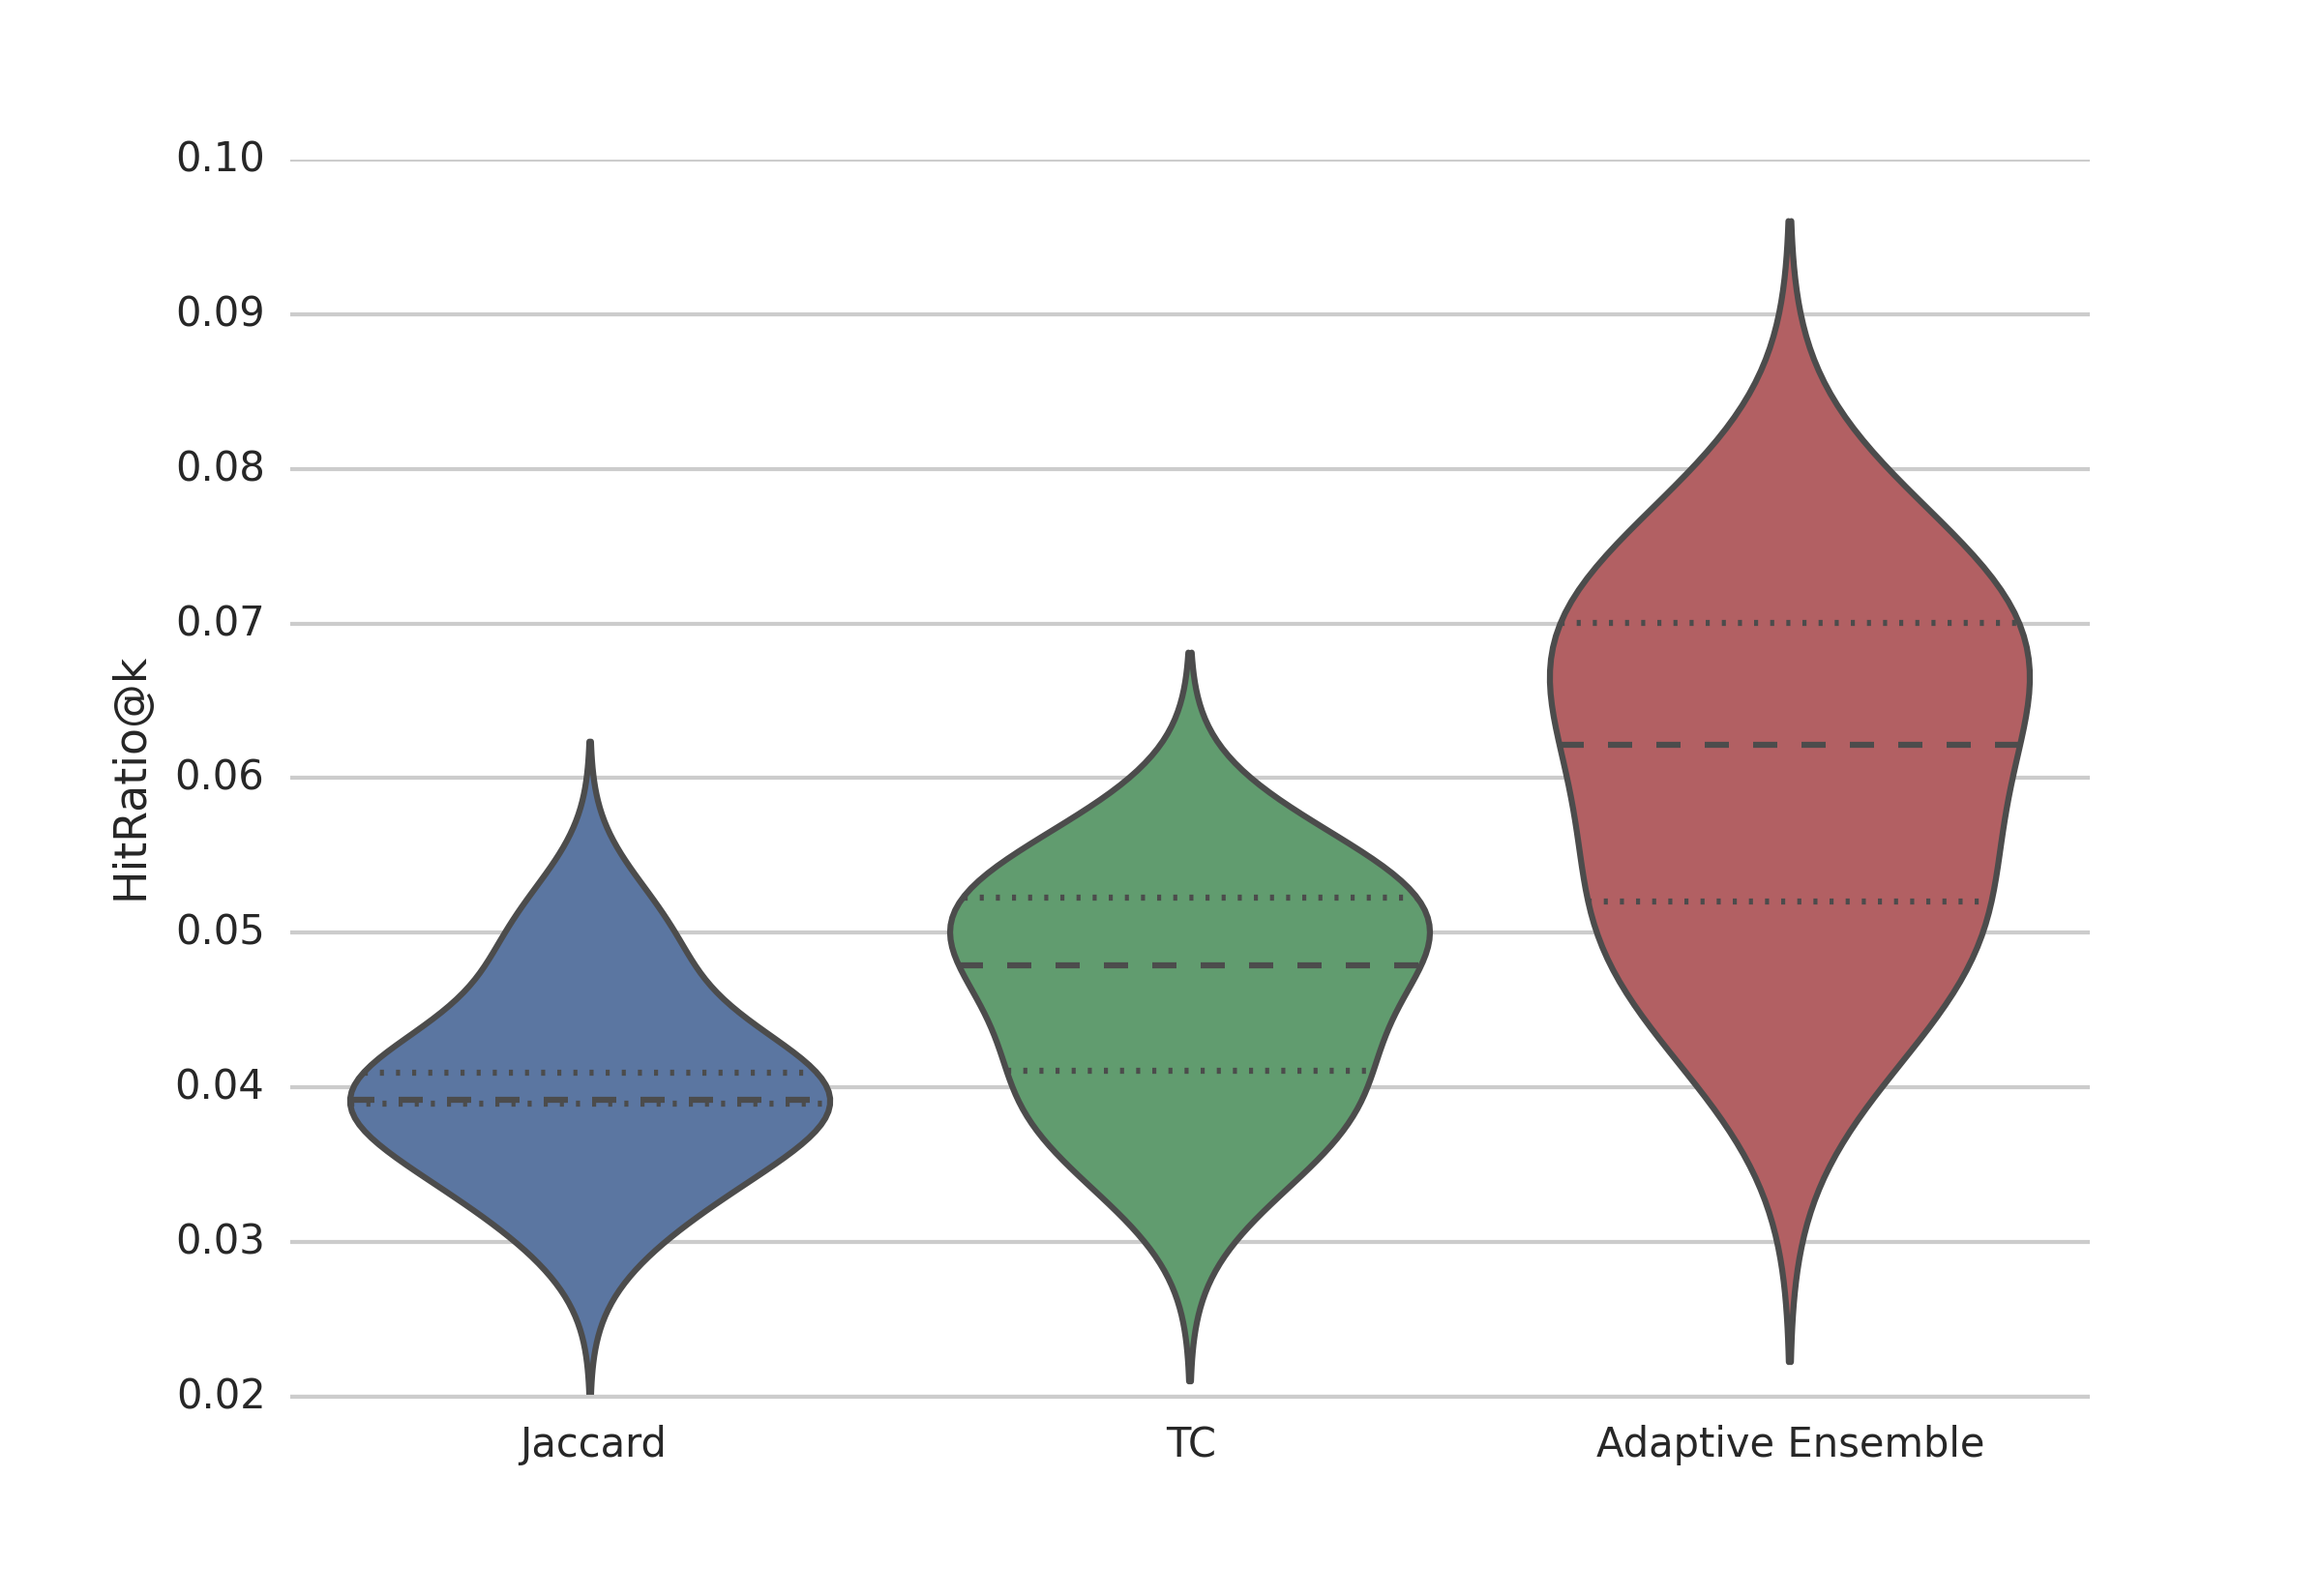
\includegraphics[width=0.95\linewidth]{images/hitratio_violin.png}
    \caption{The second subfigure.}
    \label{fig:example:subfigures:b}
  \end{subfigure}
  \caption{Demonstration of the \emph{subfigure} environment inside a figure environment}
  \label{fig:example:subfigures}
\end{figure}



\begin{figure}[htb]
  \begin{subfigure}[b]{.45\linewidth}
    \centering
    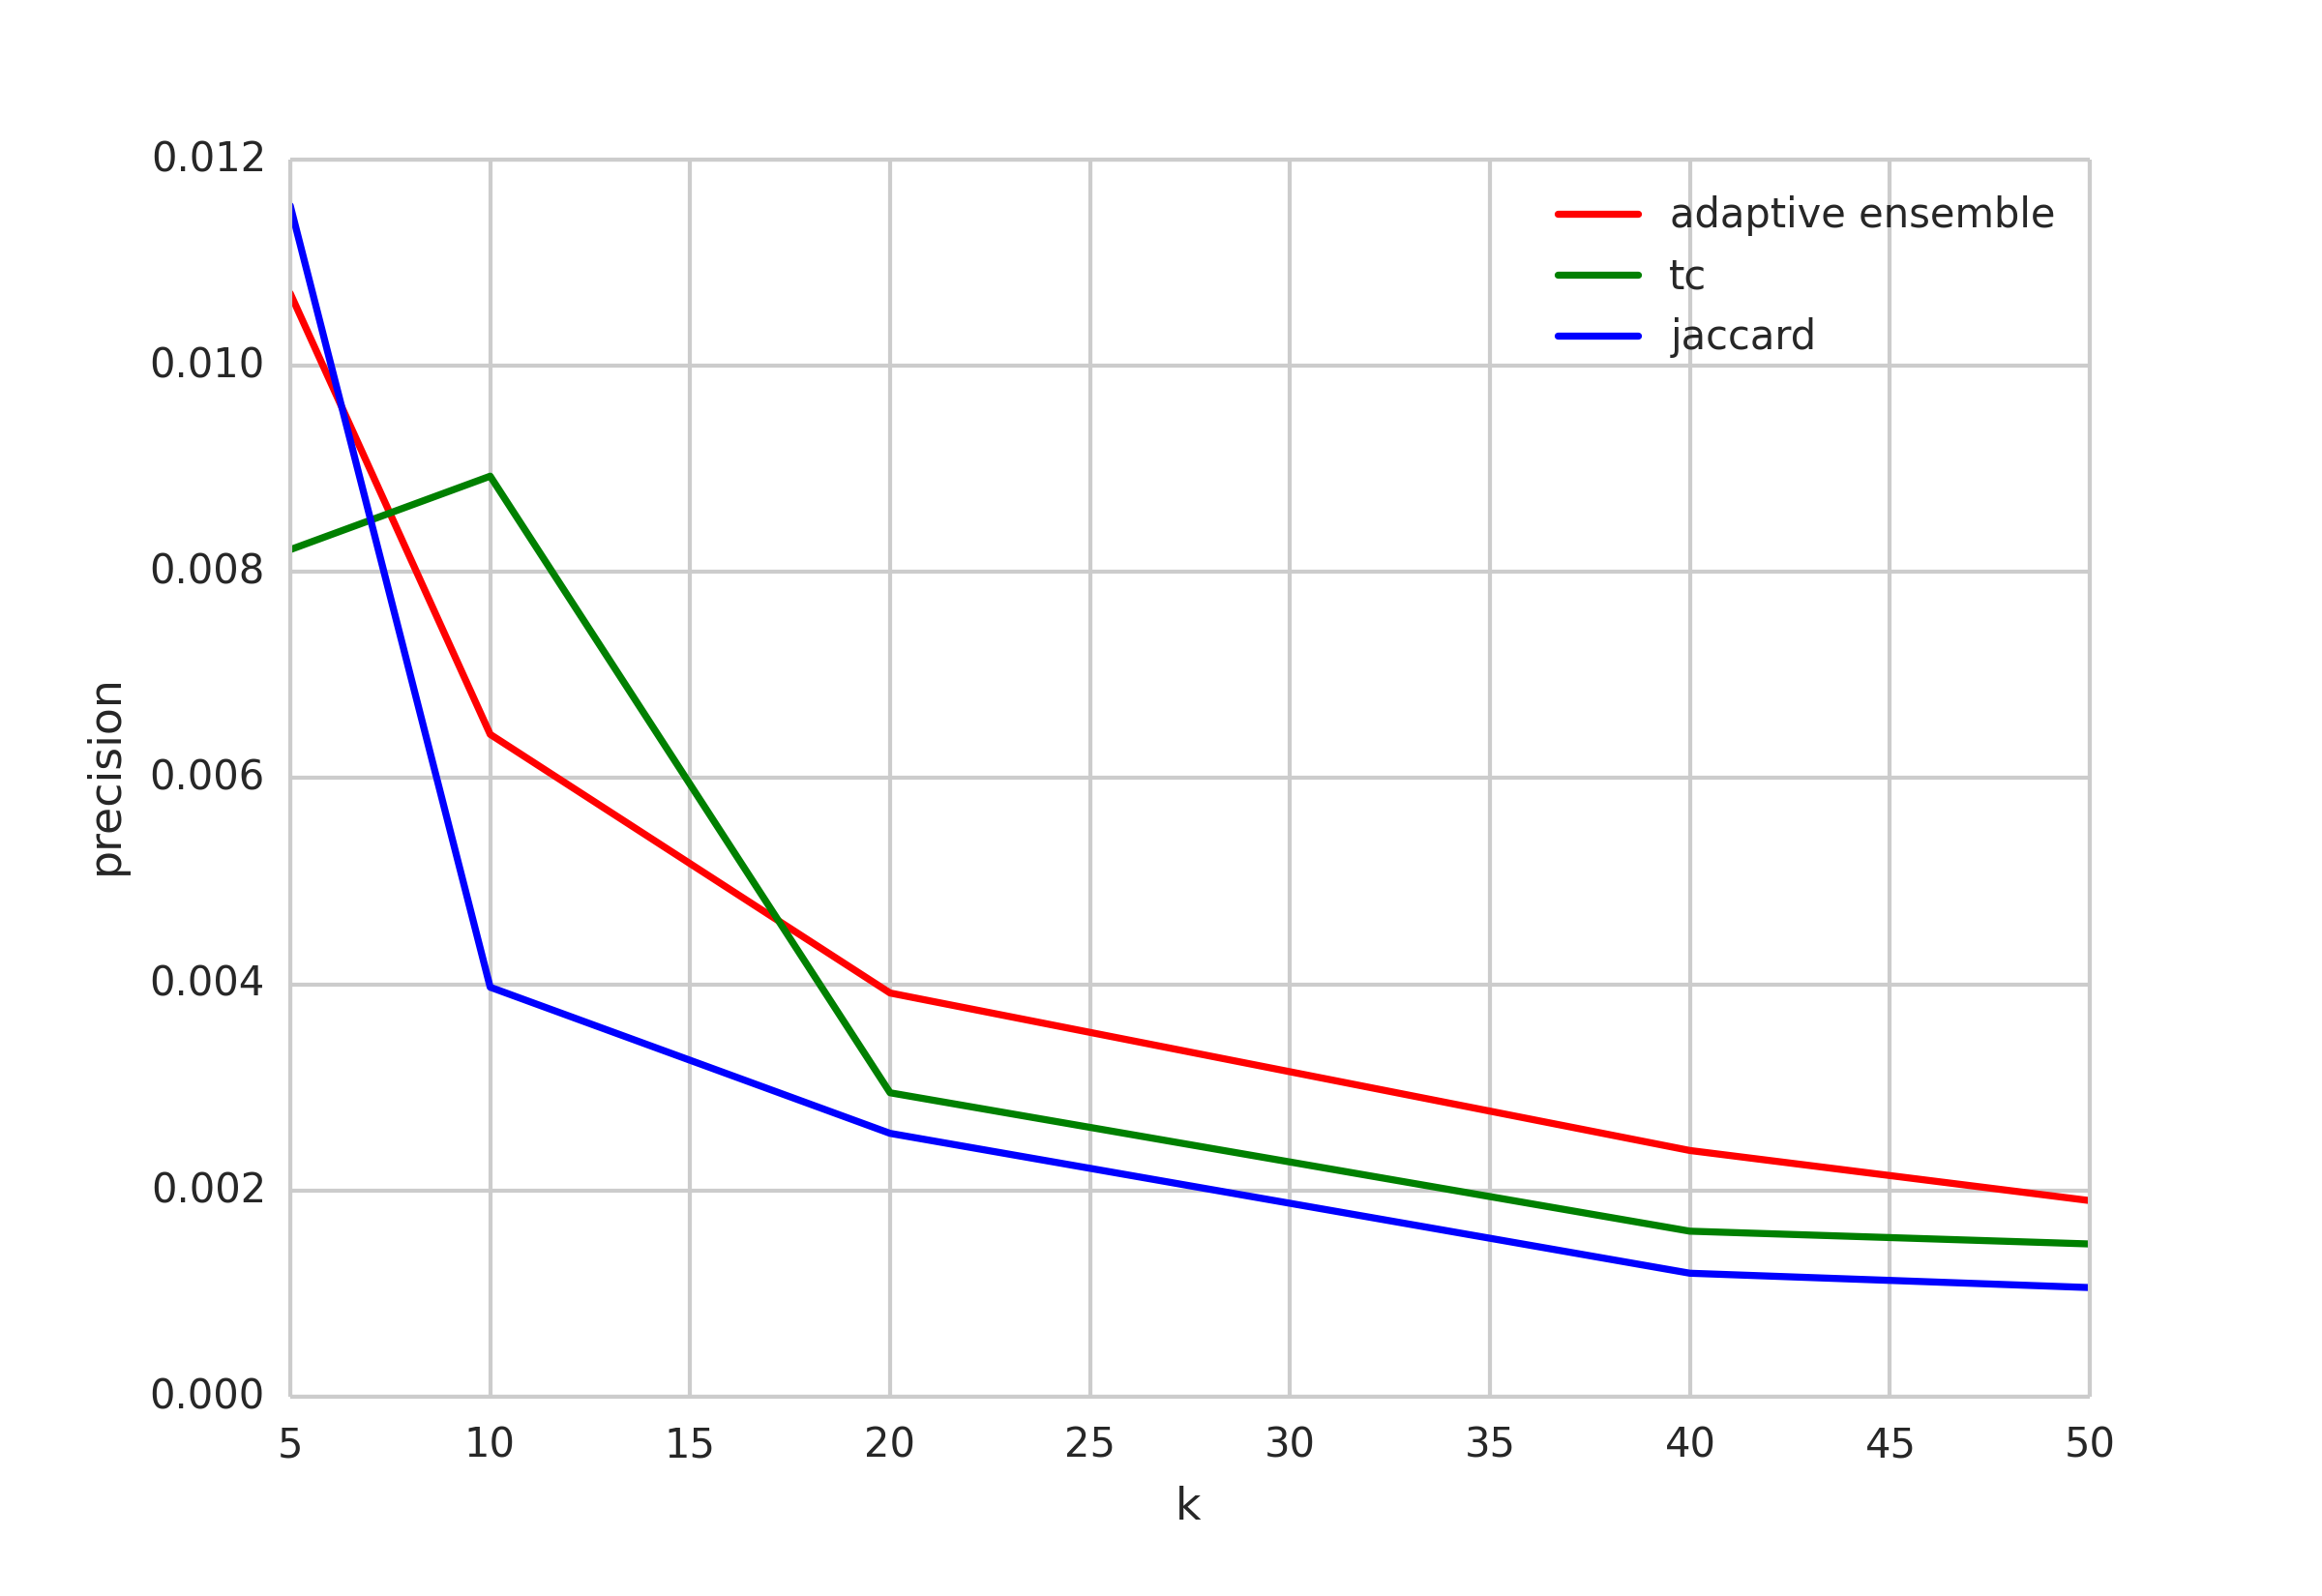
\includegraphics[width=0.95\linewidth]{images/precision_line.png}
    \caption{The first subfigure.}
    \label{fig:example:subfigures:a}
  \end{subfigure}%
  \begin{subfigure}[b]{.45\linewidth}
    \centering
    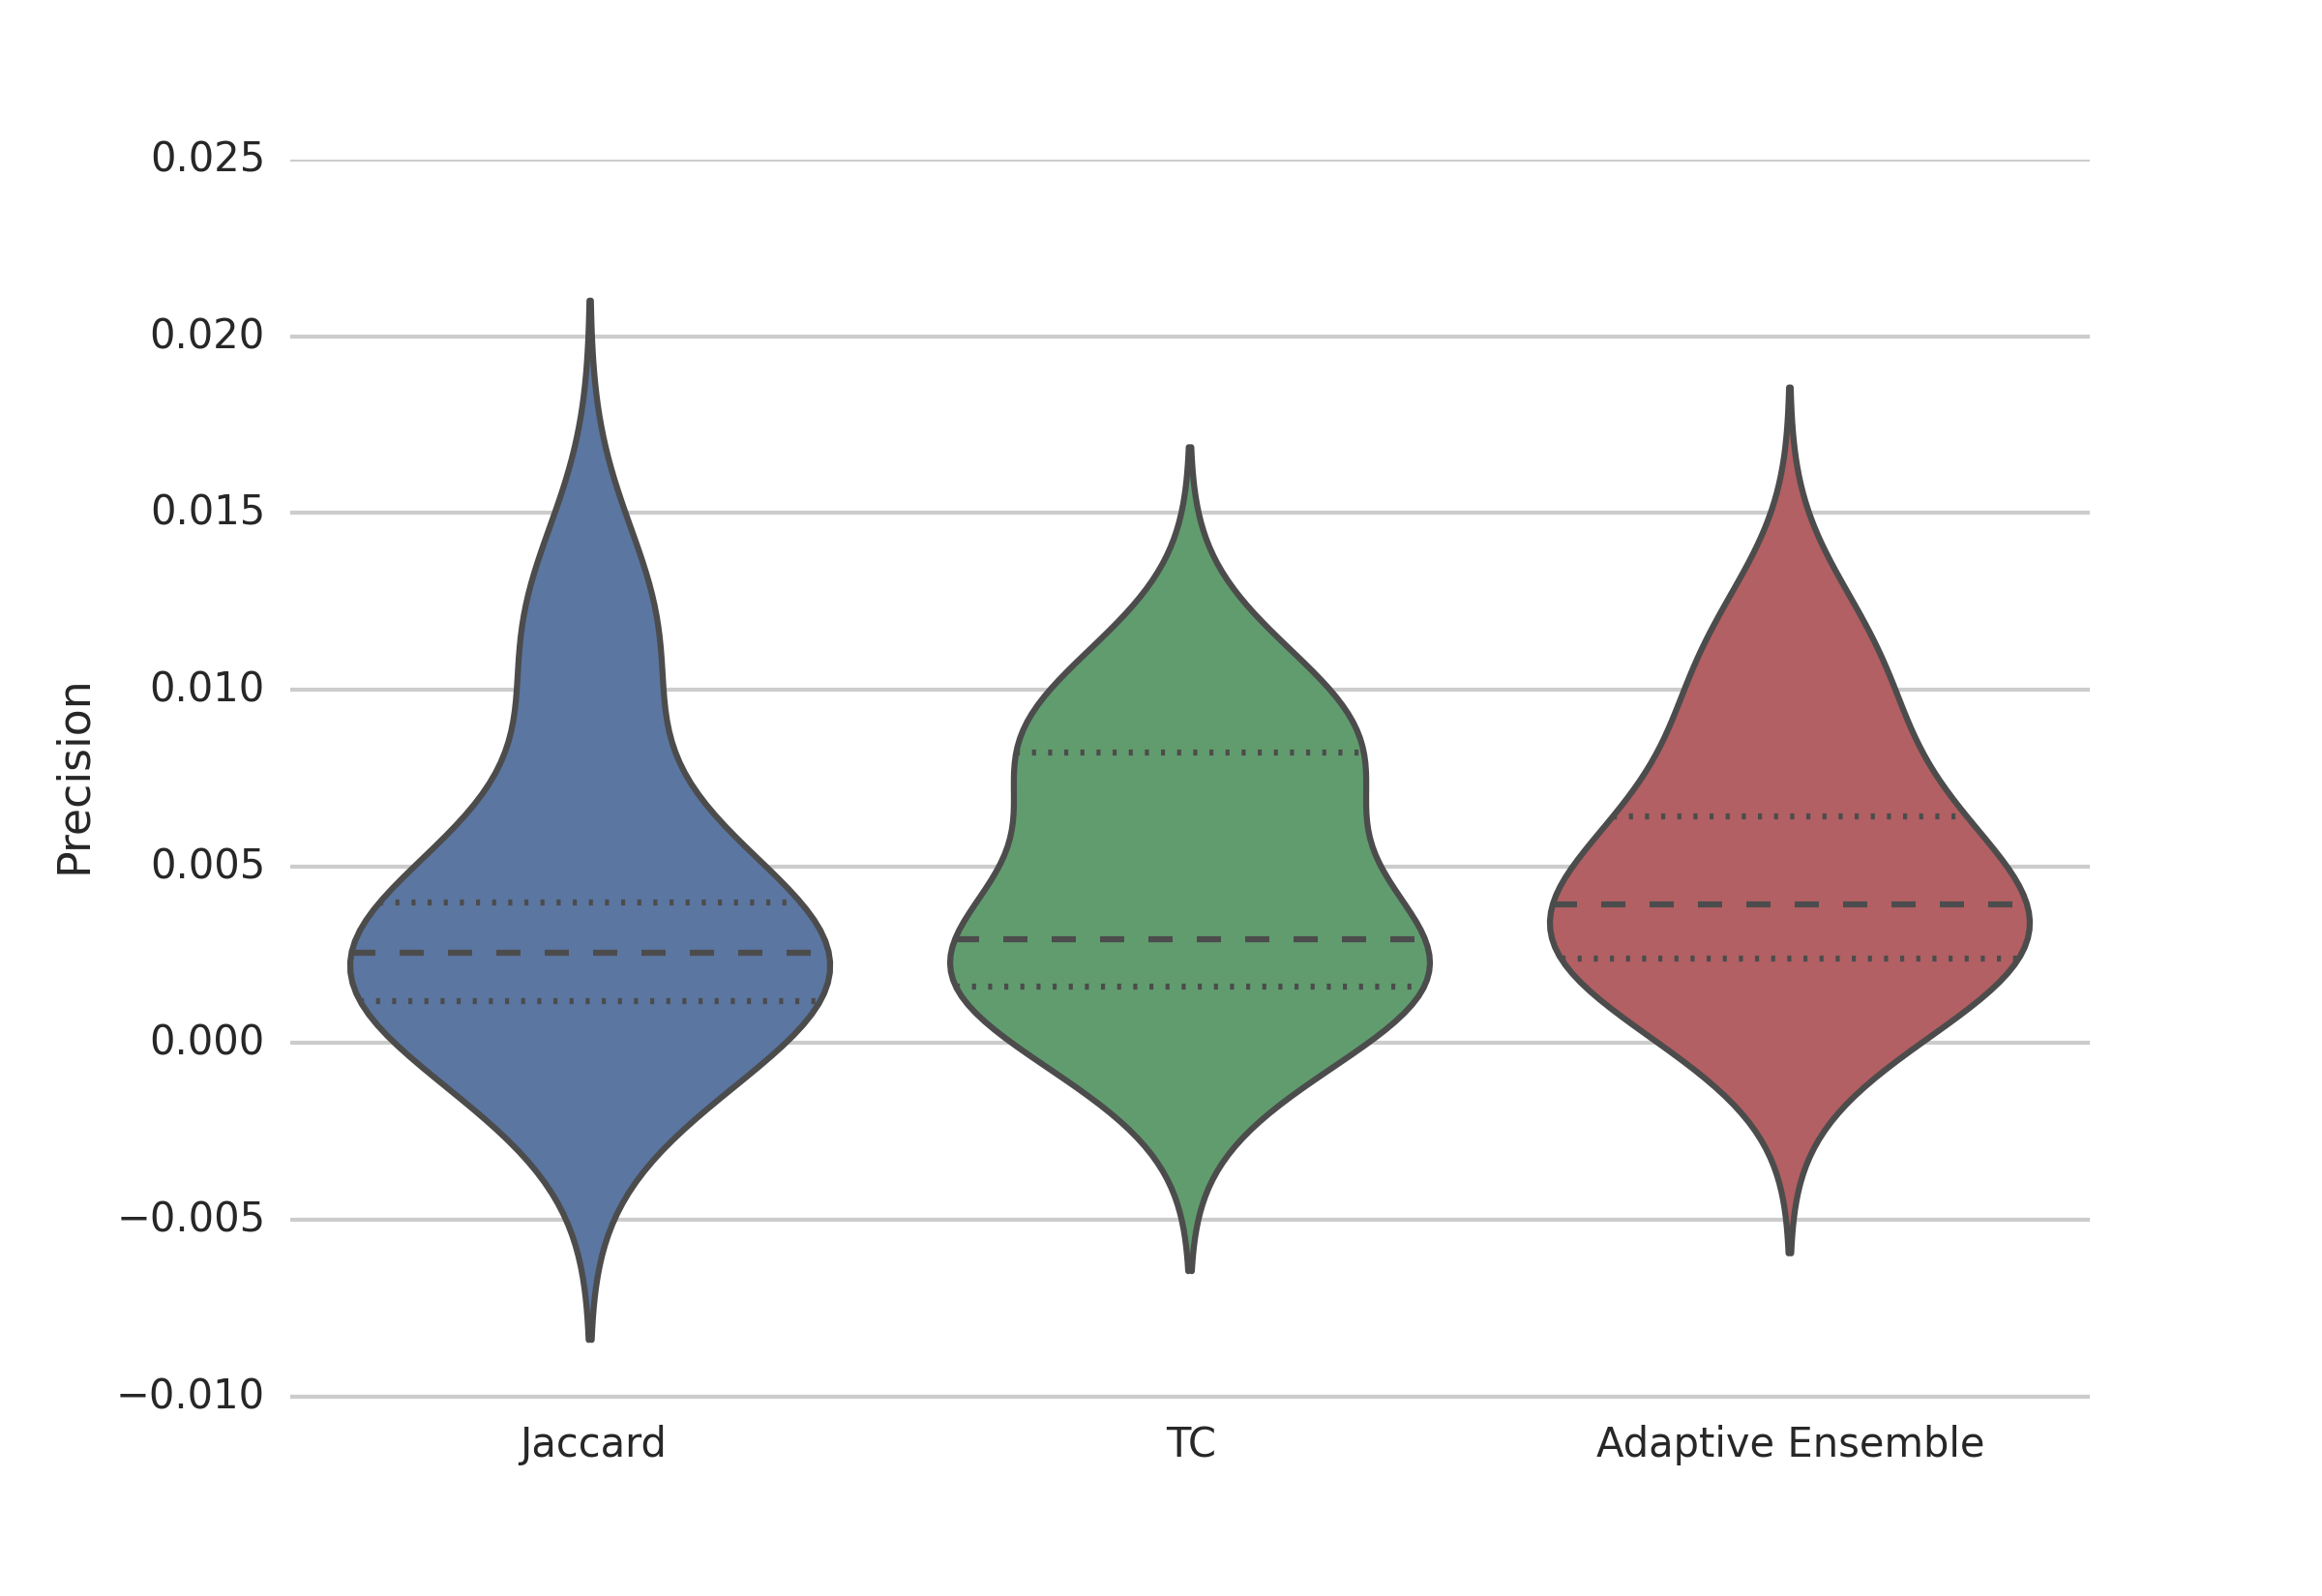
\includegraphics[width=0.95\linewidth]{images/precision_violin.png}
    \caption{The second subfigure.}
    \label{fig:example:subfigures:b}
  \end{subfigure}
  \caption{Demonstration of the \emph{subfigure} environment inside a figure environment}
  \label{fig:example:subfigures}
\end{figure}
%
For complex subfigure constructs and correct alignment of the subcaption the \texttt{floatrow} provides powerful commands. 


\subsection{Evaluation}
The system is evaluated using several iterations for cross-validation with different configurations. Table \ref{results} shows the results. Two methods of evaluation are identified as the standard for evaluating link prediction systems: precision and area under the receiver operating characteristic curve (AUC). Precision is defined as the ratio of the relevant items selected to the total number of items selected. AUC is a more involved calculation that requires an all-pairs comparison of the rank of the predicted link and {\textit all other possible unobserved links in the network}. Due to the size of the GitHub network, calculating this metric was not seen as feasible. Instead of AUC, a simple accuracy metric is calculated: if the removed link is present in the array of predicted links we count the test run as correct, if not we consider it incorrect. Accuracy is therefore the number of correct predictions divided by the total number of runs. Due to the large number of possible links we expect these accuracy metrics to be quite low, relative to other recommender system results. 

\section{Discussion}
Table \ref{results} details the results of running our algorithm for various configurations of the parameters k and n, where k is the number of neighbors considered to generate recommended links and n is the number of predicted links generated for each user. We calculate both precision and accuracy for each run, where accuracy is defined as the number of users for which the removed link was observed to be in the set of predicted links divided by the total number of users in that run. In other words, we count a prediction as "correct" if v, the removed {\textit FOLLOWS} edge is in the set of predicted edges. Using this same definition of correctness, we calculate the probability of accuracy if the links were chosen at random from our graph of existing GitHub users. We can see that for almost all configurations, the results are significantly (approximately 3000X) better than choosing links at random. Surprisingly, the best performing configurations (as measured by both accuracy and precision) are those with the lowest values of K (the number of neighbors used to generate recommendations).


